\lab{Applications}{PageRank Algorithm}{PageRank Algorithm}
\label{Ch:PageRank}

\objective{Explain the basics of the PageRank Algorithm, and some of its applications}

The PageRank Algorithm is core algorithm used by Google to classify search results. It is based upon an interesting mathematical model that involves random processes, Markov chains and eigenvalues. It ranks pages webpages based upon their connectivity properties with the rest of the web. When you make a query on Google's webpage they find every webpage that contains the keywords you specified and then list them primarily in order of page rank (this isn't true in every case, but it is generally how it works).

The PageRank Algorithm works by supposing that a person surfing the internet randomly clicks links on the webpages. We will notate the probability that the surfer is a particular page $i$ at time $t$ by $PR(i,t)$. We can write an equation for this probability from one time step to the next using the following notation:
\[
PR(i,t+1) = \sum_{j \in M(i)} \frac{PR(j,t)}{L(j)}
\]

Where $M(i)$ is the set of pages that link to page $i$, and $L(j)$ represents the number of outbound links on page $j$. Note that this is simply representing the internet as a markov chain, just like we discussed in Lab \ref{Markov}. We assume that the starting probability is uniform, or in other words that $PR(i,0) = 1/N$.

However, there are two minor modifications that we make to this formula. First, what if a page has no outbound links? In this case we pretend that the page links to every other page (as if the surfer, upon getting stuck, randomly picks a new page). Second, we assume that the surfer sometimes gets bored and randomly picks a new page. The probability that the surfer doesn't get bored is called the damping factor $d$ and is usually set to $.85$. Using these modifications we can write our formula as:
\[
PR(i,t+1) = \frac{1-d}{N} + d\sum_{j \in M(i)} \frac{PR(j,t)}{L(j)}
\]

Note that $N$ is the total number of webpages. We then say that the page rank of a particular webpage is the value
\[
PR(i) = \lim_{t\to \infty} PR(i,t)
\]

Mathematically therefore, the page rank is the steady state probability of our modified Markov chain. We can rewrite this as a matrix equation:
\[
R(t+1) = d K R(t) + \frac{1-d}{N} \begin{pmatrix}1\\\vdots\end{pmatrix}
\]

Where $R_i(t) = PR(i,t)$. The matrix $K$ is defined by:
\[
K_{ij} = \begin{cases} \frac{1}{L(j)} & \mbox{ if j is linked to i} \\ 0 & \mbox{ otherwise} \end{cases}
\]

We can write $K$ neatly as follows:
\[
K = (B^{-1}A)^T
\]

Where $A$ is the adjacency matrix for the directed graph (the edges are links) and $B$ is the diagonal matrix containing the outdegree of each vertex\begin{matlab} (i.e. \li{diag(sum(A'))})\end{matlab}. Recall that we have to modify our graph so that any page without outbound links points to every other page, otherwise these definitions don't make sense (for example $B^{-1}$ will not be well-defined).

There are several ways to solve for $\lim_{t \to \infty} R(t)$. One option is simply iterate the equation until $\norm{R(t)-R(t-1)}$ is sufficiently small. Another option is to instead assume a steady state (i.e. $R(t) = R(t-1)$) giving the equation:
\[
R(t+1) = d K R(t) + \frac{1-d}{N} \begin{pmatrix}1\\\vdots\end{pmatrix}
\]
Which we can then reduce to the following form solvable by least squares:
\[
(I-dK)R = \frac{1-d}{N} \begin{pmatrix}1\\\vdots\end{pmatrix}
\]

A third option is available. Since $R$ can be viewed as a vector of probabilities we can rewrite $\left(\begin{smallmatrix}1\\\vdots\end{smallmatrix}\right) = E R$, where $E$ is a matrix of all ones. Thus the equation becomes:
\[
R = (dK + \frac{1-d}{N}E)R
\]
Since $(dK + \frac{1-d}{N}E)$ will be a strictly positive stochastic matrix (each column sums to one) we can use the Perron-Frobenius theorem to guarantee that this eigenvalue equation corresponds to the largest magnitude eigenvalue and that the eigenvector is unique. Thus by finding the eigenvector corresponding to the largest eigenvalue of $(dK + \frac{1-d}{N}E)$ we can find $R$. This can be found relatively easily using the power method as in lab \ref{Ch:EigSolve}. It actually turns out that the first option for finding $R$ (the iterative approach) is essentially equivalent to the eigenvalue approach.

Once we have calculated $R$ we are done. $R$ gives the page rank associated with each webpage. A useful way to think of this algorithm is to think in terms of voting. Every link that I place on my webpage is a vote for the webpage that it points to. Additionally, if I am more prestigious then my votes count for more.

This algorithm has been used in several settings (primarily in academia). For example, it has been used to rank graduate institutions, to rank impact factor of journals and has even been used in some biological applications.

Let's try implementing the PageRank algorithm on a small subset of the internet. The file \li{internet.dat} contains the connections between webpages on all of the websites supported by Notre Dame University in the year 1999 ({\bf We might need permission to use this file...also need a link}). We can load this data to a sparse matrix using the following:

\begin{matlab}
\begin{lstlisting}[style=matlab]
load internet.dat;
internet(:,1:2) = internet(:,1:2) + 1;
A = spconvert(internet);
\end{lstlisting}

The second line is necessary because the numbering of webpages started at $0$ instead of $1$ in the original data file. The \li{spy} command of this adjacency matrix yields the plot shown in figure \ref{Fig:WebSparse}
\end{matlab}

\begin{python}
\begin{lstlisting}[style=python]
: internet = sp.load("internet.npy")
: A = spconvert(internet)
\end{lstlisting}
The \li{matplotlib.pyplot.spy} command of this adjacency matrix yields the plot shown in figure \ref{Fig:WebSparse}
\end{python}


\begin{figure}
\begin{center}
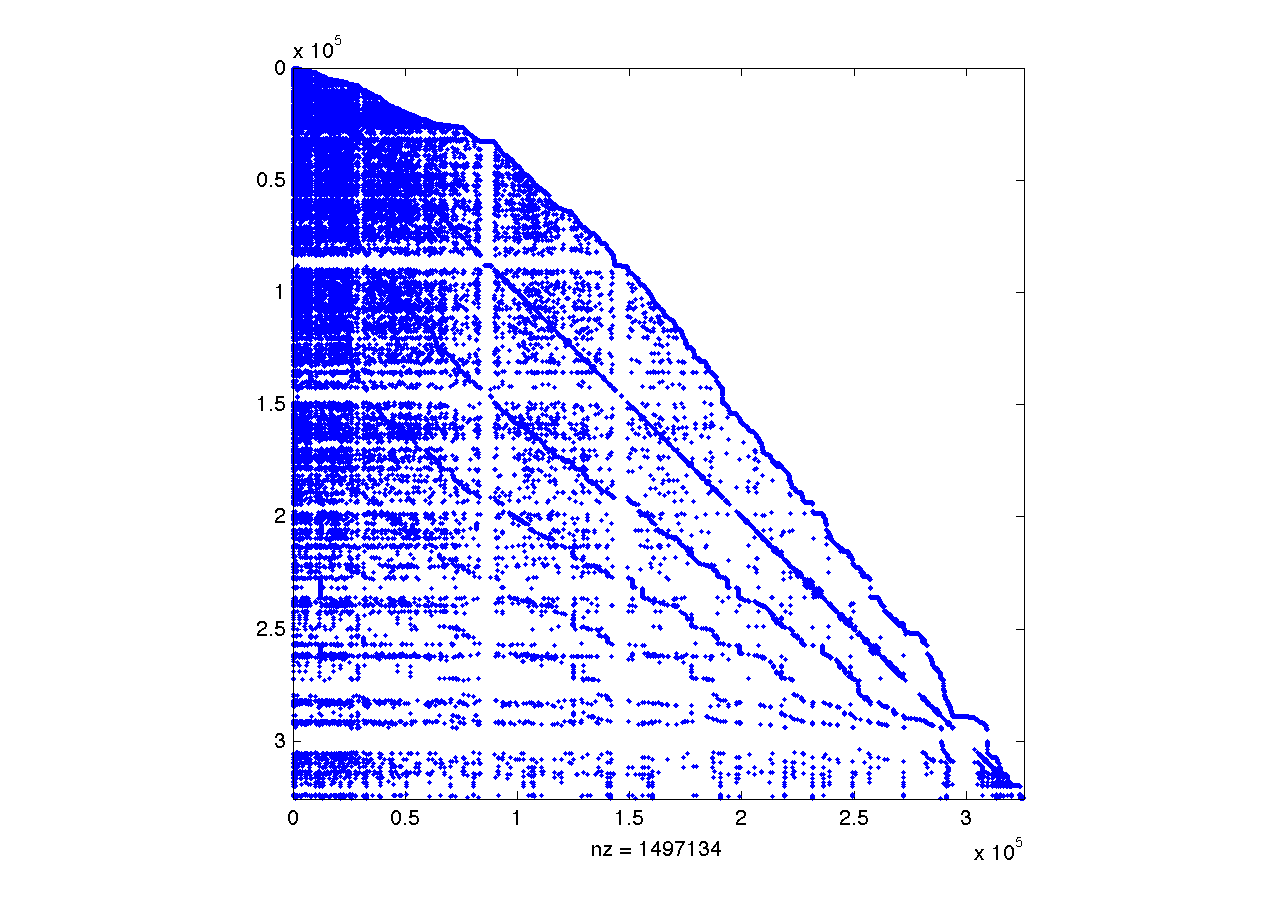
\includegraphics[scale = .4]{./Figures/WebSparse.pdf}
\caption{\li{spy} command on the adjacency matrix corresponding to a portion of the internet}
\label{Fig:WebSparse}
\end{center}
\end{figure}

\begin{problem}
\label{prob:pg_undirected}
A directed graph is called weakly connected if the associated undirected graph (the graph obtained by replacing all directed edges by undirected ones) is connected. Use the eigenvalues of the graph laplacian to determine whether the graph representing this portion of the internet is weakly connected (refer to lab \ref{Ch:EigGraph} if you don't remember how to do this).
\end{problem}

\begin{problem}
\label{prob:pg_calc}
Calculate the PageRank on the first 6000 webpages in the data set. Remember that first you must set any rows that are all zeros to be rows of ones. Which page has the highest page rank, and what is the value of the page rank? Which method works the best? Why?
\end{problem}
%Solution: page number 1, .0643

\begin{problem}
The iterative method allows the easiest implementation for large-scale problems (everything can be done using sparse matrices). Using an implementation that uses only sparse matrices, calculate the PageRank on the entire set of webpages. Which page has the highest page rank, and what is the value of the page rank?
\end{problem}
%Solution: page number 1964, .0055

